\section{Introduction}
\label{introduction}
VTK is an open source cross-platform software system used for scientific data
processing, analysis and visualization. It was originally developed to provide
examples accompanying a book on object oriented computer graphics
programming~\citep{schroeder_visualization_2006, geveci_vtk_2012}.  Since its
inception, VTK has a long history of volume rendering and, unfortunately, that
history is evident in the large selection of classes available to render
volumes. Each of these methods was state-of-the-art at the time it was
introduced, but given VTK's 20+ year history, many of these methods are now
quite obsolete. Recently, there has been a major
effort~\citep{hanwell_visualization_2015} undertaken to re-write the rendering
backend from using legacy deprecated OpenGL API to a more modern programmable
pipeline based OpenGL API~\citep{shreiner_opengl_2013}, to support latest
technological advances in the graphics hardware industry. One of the goals of
this work was to reduce the number of volume mappers to ideally just two: one
that supports accelerated rendering on the Graphics Processing Unit (GPU) and
another that works in parallel on the Central Processing Unit (CPU). The
\texttt{vtkSmartVolumeMapper} would help application developers by automatically
choosing between these techniques based on the system configuration.

\begin{figure}[ht]
  \centering
  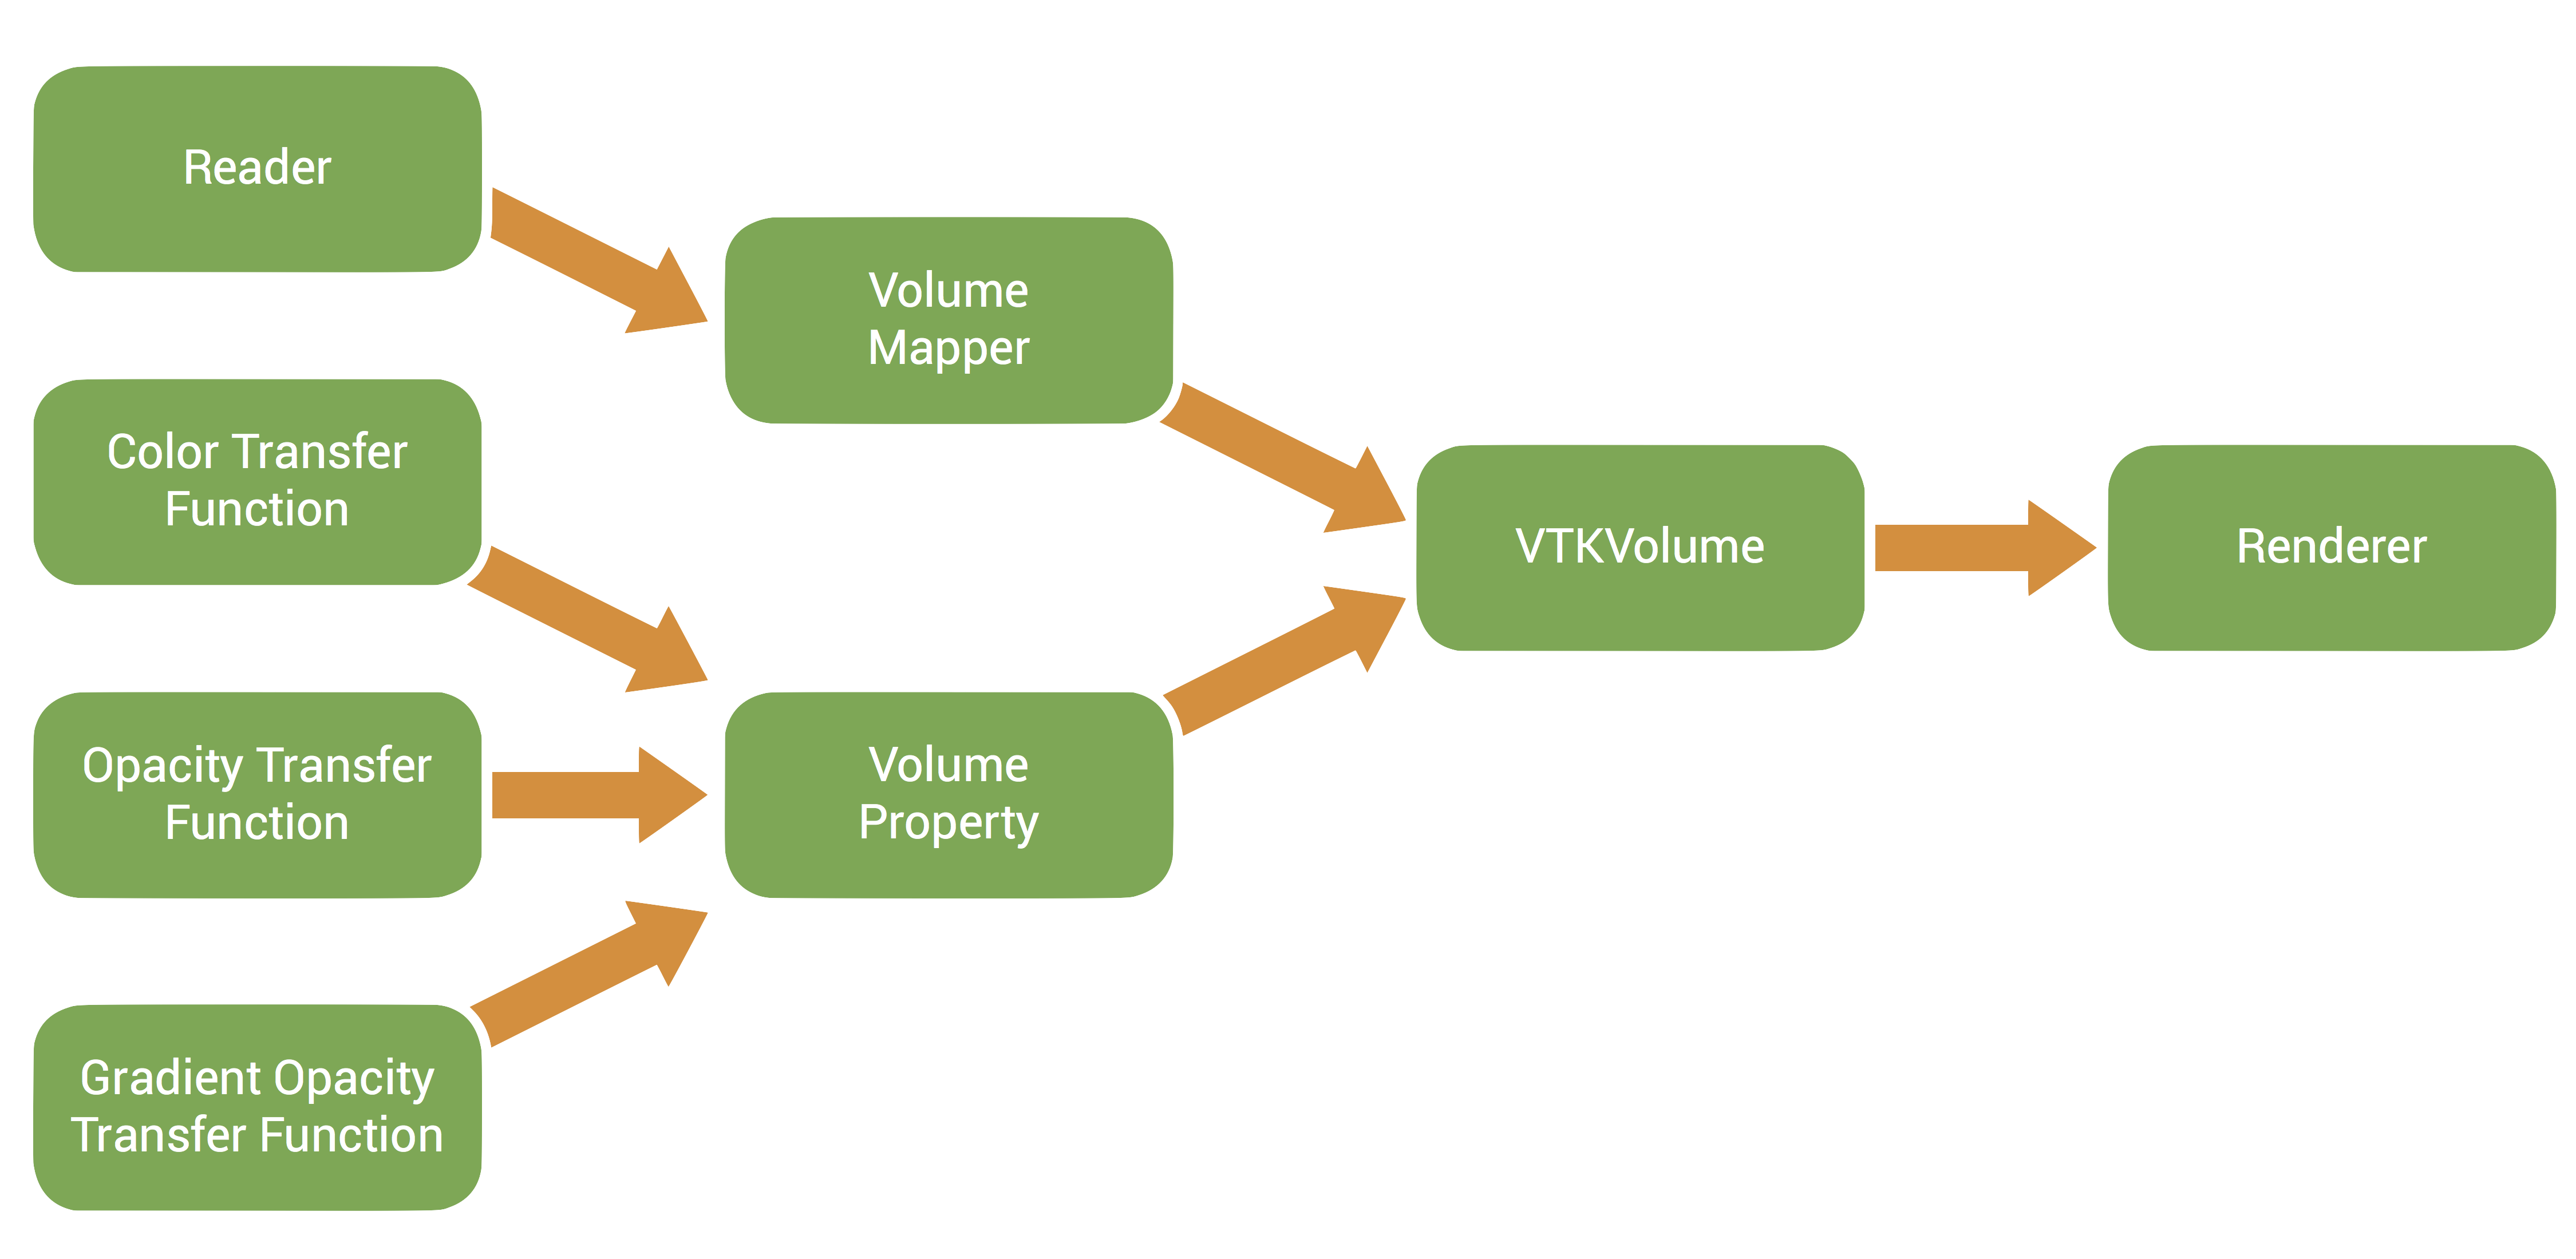
\includegraphics[width=\columnwidth]{vtk_volume_pipeline.png}
  \caption{VTK pipeline for volume rendering which is similar to VTK polygonal
    rendering with differences such as transfer functions are defined on the
    property object.}
  \label{fig:pipeline}
\end{figure}%

The main objective of this effort is to create a cross-platform,
multi-functional and high-performance volume renderer that works in both serial
and parallel mode (for example in
ParaView~\citep{ahrens_paraview:_2005,ayachit_paraview_2015}). Our volume
visualization effort is novel in the following way:

\begin{itemize}
  \item The new volume visualization supports all major operating
    systems and compute environments (Desktop, VR, Mobile) and performs equally
    well on all the systems.

  \item The new volume visualization supports a VTK-based pipeline and data-flow
    networks that provide a highly flexible system for scientific and medical data
    visualization use-cases.

  \item Our technique supports a variety of useful features at interactive frame
    rates such as Clipping, Cropping, Gradient Opacity, Geometry-Volume translucent
    rendering and on demand shader composition.
\end{itemize}

To achieve this, we have created a replacement for the OpenGL fixed pipeline based
vtkGPUVolumeRayCastMapper. The new mapper, which shares the same name but uses
the OpenGL programmable pipeline, can be used via \texttt{vtkSmartVolumeMapper} or
instantiated directly and replaces the old \texttt{vtkGPUVolumeRayCastMapper}.
Availability of the new mapper with new OpenGL-VTK implementation improved the
management of textures in the mapper and benefited both forms of rendering
(geometry and volume) by sharing common code between them. While volume
ray-casting itself is a well-known technique, developing a volume renderer that
works with variety of data formats and types, supports many essential features
for medical and scientific computing, works on the main commercial platforms
(such as Windows, Mac, and Linux) and performs well at interactive frame rates
with very large datasets is still a challenging task that requires an in-depth
knowledge of the data, graphics pipeline, the VTK framework and the user
requirements.  In the next section, we will cover technical details of our work
that resulted in a sophisticated volume renderer for the VTK community.
